\documentclass[12pt,a4paper]{article}
%
% Note: if writing in Finnish, modify commented lines in this file properly.
%
\usepackage{amsmath,graphicx,float,times}
\usepackage[english]{babel} % if writing in Finnish, replace english with 'finnish'.
\usepackage[T1]{fontenc}
\usepackage{cite,url}
\usepackage{ae,aecompl}
\usepackage{color}
\usepackage{uefreport_short} % some local definitions

% My Packages
\usepackage{subcaption}
\usepackage{siunitx}
\usepackage{hyperref}
\hypersetup{colorlinks=true,linkcolor=blue,citecolor=red,urlcolor=cyan,breaklinks=true}
\usepackage{pdfpages}
%
\begin{document}
%
\begin{frontmatter}
%
% Title of the work
%
\title{Simulation and Analysis of Fields in a High Numerical Aperture Lens} % Remove this after reading ;)
%
% Author(s). Separate multiple authors with comma, second to last and last with "and".
%
\authors{Charles Rambo}
%
% Corresponding addresses. Use \\ command to break line wherever necessary
%
University of Eastern Finland, Master's Degree Programme in Photonics\\[1mm]
%
% Supervisor(s)
%
Supervisor: Dr. Xiaorun Zang
%
\email{chrambo@student.uef.fi} % e-mail address of the corresponding author
%
\uefabstract{In this work, the process of using an objective lens with a high numerical aperture (N.A.) to focus a vector beam is outlined. Numerical methods are then performed via a Python-based simulation allowing for the lens to be evaluated under a variety of conditions. The result of these simulations are presented and the data is analysed in various ways using Python. The analysis showed that all beams tested lead to a toroidal intensity profile resembling a Laguerre-Gaussian $lm$ mode where the radial index $l\neq 0$. The polarization of resulting field follow the input polarization and has an important impact on the intensity of the field in the focal region. Changes in wavelength showed that beams with a shorter wavelength will result in a more tightly focused field. Also, N.A. was varied and showed that the results of the simulation are reasonable.}
%
\end{frontmatter}
\thispagestyle{empty}
\tableofcontents
\clearpage
%
\pagestyle{plain}
\setcounter{page}{1}
%
\section{Introduction}
%
It is of course well known that the invention of the microscope by Robert Hooke (pictured on the title page) ushered in a new scientific frontier in observing the universe up close that would go well beyond fleas and cell structure. One particular advance in microscope design was the development of a single value to describe the light-gathering power of a lens known as the numerical aperture (N.A.) by Ernst Abbe, who realized that there was an inherent connection between wavelength, N.A. and resolving power of a microscope \cite{Hecht}. For a long time, the limit for the resolving power of a lens was believed to be much higher than what is now considered to be the threshold as the beam being used had been a scalar Gaussian beam \cite{Novotny}. A vector beam with a radial electric field vector is may be focused by a high N.A. lens to a smaller spot size than a typical scalar Gaussian beam which is why they are applied in high-resolution microscopy\cite{Saleh}. 

The result of considering the focal field of a vector beam passing through a high N.A. lens is a set of complex equations, and further, these equations must be solved across the range of angles accepted by the lens aperture otherwise the results do not have much meaning. These complications mean that many calculations must be carried out and it is therefore much more sensible to apply numerical analysis to simulate the beam through the system. In this work code for the simulation of vector beam passing to the focal region of a lens has been written in Python, which served the purpose of allowing a multitude of beam and lens conditions to be considered, and compared against each other.

In the next chapter the concepts behind resolving vector beams in a high N.A. lens, in the third chapter the techniques for data collection are explained. The collected data is then analysed and discussed in the fourth chapter, which leads to the conclusions presented in the end where it is shown that when a beam is passed through even an idealized high N.A. lens, one should give particular consideration to the incident polarization, which may also be measured after the lens, and that the wavelength of the beam and field profiles also play key roles in how the beam will be resolved.
%
\section{Theory}
In order to develop a simulation of for the tight focusing of the vector beam, it is important to first establish the equations that govern the process.
\begin{figure}[htb]
\centering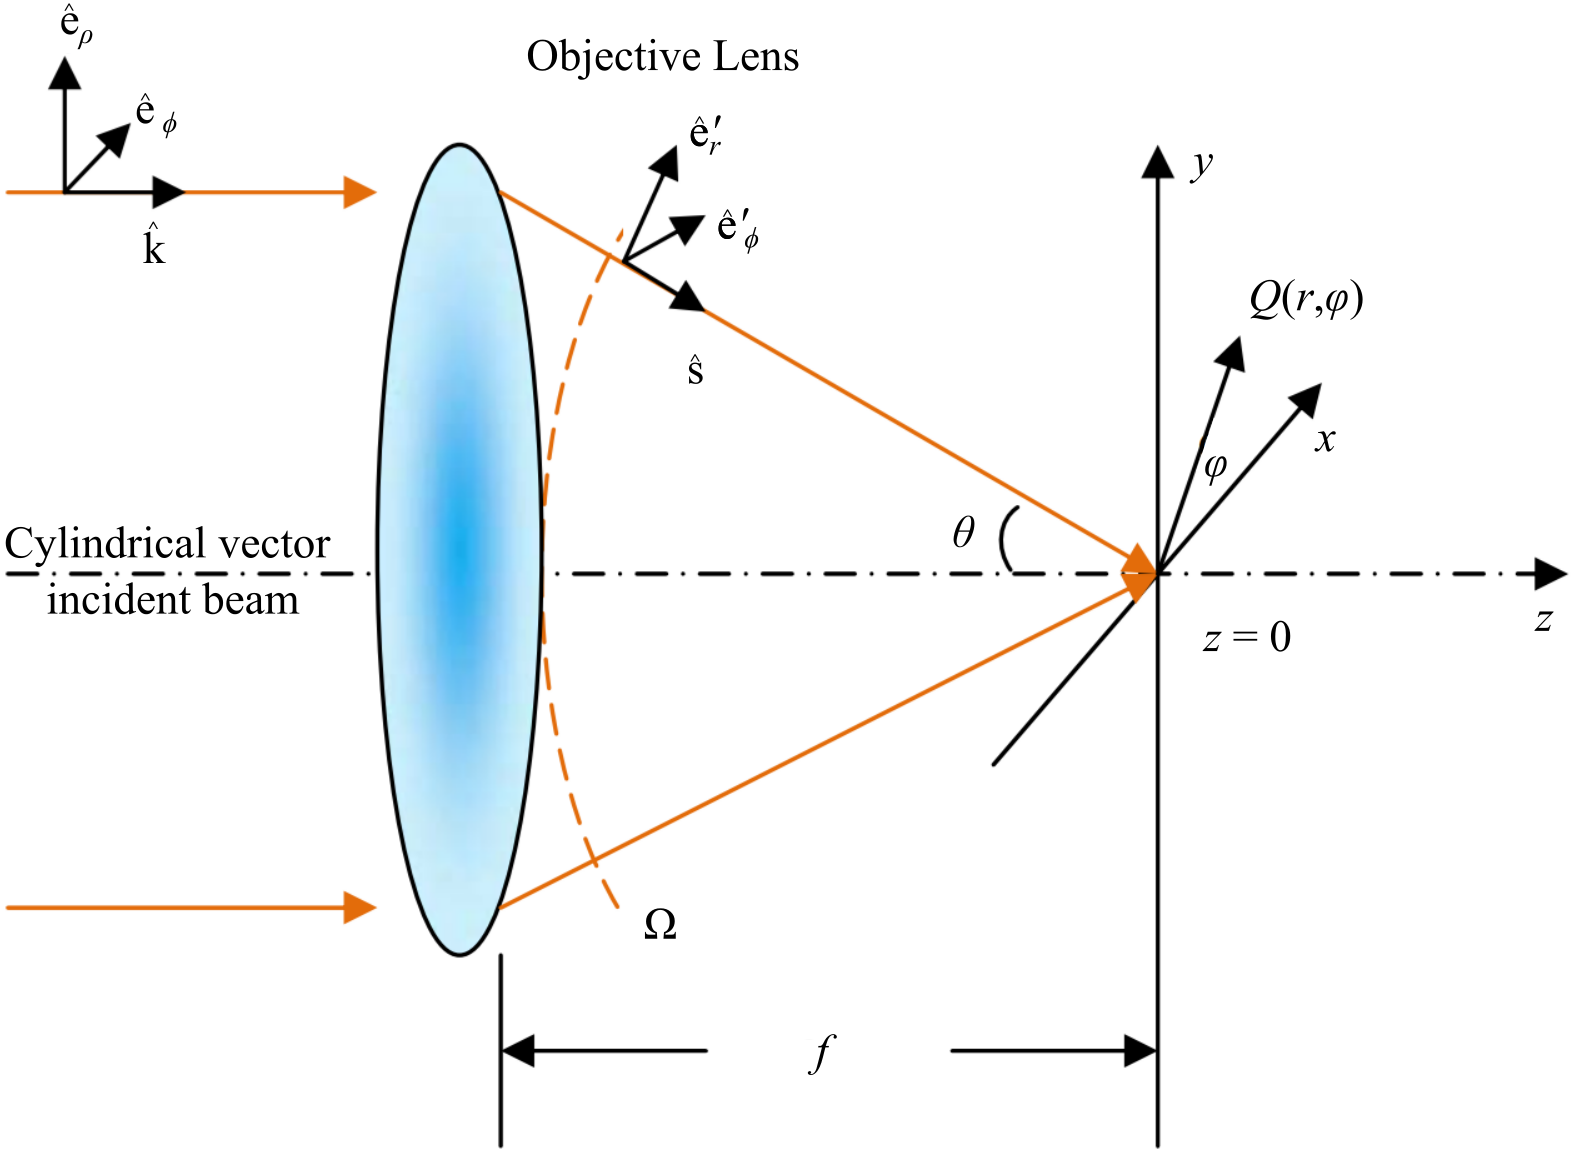
\includegraphics[width = 0.6\textwidth]{Lensdiagram}
\caption{Diagram of high N.A. lens \cite{Zhan}. The vector notation has been changed slightly for this for this work.}
\label{fig:LensDia}
\end{figure}
\subsection{Incident Vector Beam}
Using the coordinate system from Fig. \ref{fig:LensDia}, the equation in cylindrical coordinates for the radial vector beam incident along the optical axis may be written as,
\begin{equation}\label{start}
\textbf{E}(\rho, \varphi) = l_0P(\rho)[\cos\varphi_0 \hat{\textbf{e}}_\rho+\sin\varphi_0\hat{\textbf{e}}_\varphi].
\end{equation}
Here, $P(\rho)$ is the radial field profile for the incident beam and $l$ is the peak field amplitude which normalizes $P(\rho)$. The 0 subscript indicates incidence. The field profile may be practically any function, which will then be taken to be symmetric about the $z$ axis. In most of the following simulations, the Gaussian field defined by 
\begin{equation}
P(\rho) = \exp[-\rho/w)^2]
\end{equation}
is used here, which results in the LG$_{00}$ mode, $w$ is the waist of the beam, and it will more or less controls the beams radial extension. As it would be inefficient to bother calculating regions of the lens where the beam is not incident, the waist of the beam was set relative to the acceptance angle $\theta_\text{max}$ which will be defined momentarily as
\begin{equation}
\label{eqn:beamwaist}
w = f\sin\theta_\text{max}.
\end{equation}

\subsection{Propagation Through the System}
Upon propagating through the lens, the beam profile is mathematically mapped to an apodization function that is converging angle $\theta$-dependent. Mapping the LG$_{00}$ mode through this process yields
\begin{equation}\label{eqn:Ptheta}
P(\rho)\mapsto P(\theta) = P(f\sin\theta)\sqrt{\cos\theta} \Rightarrow \exp[-(f\sin(\theta)/w)^2]\sqrt{\cos\theta}.
\end{equation}
Of course the polarization should also be considered. The affect of the propagation on the polarization is,

\begin{equation}	\label{eqn:Pol}
	\begin{aligned}
	\hat{\textbf{e}}'_r & = \cos\theta \hat{\textbf{e}}_\rho + \sin \hat{\textbf{e}}_z, \\
	\hat{\textbf{e}}'_\varphi & = \hat{\textbf{e}}_\varphi. 
	\end{aligned}		
\end{equation}

Substituting Eqs. \ref{eqn:Ptheta} and \ref{eqn:Pol} into \ref{start} yields the field on the reference sphere $\textbf{a}$ defined as
\begin{equation}
\textbf{a}(\theta, \varphi) = l_0fP(\theta)[\cos\varphi_0 \hat{\textbf{e}}'_r + \sin\varphi_0 \hat{\textbf{e}}'_\varphi].
\end{equation}

\subsection{The Focal Field}
Finally, the vector field on the reference sphere will be integrated by the Richards Wolf vector diffraction theory such that
\begin{equation}
\textbf{E}(r, \phi, z) = \dfrac{-ik}{2\pi} \int_{0}^{\theta_\text{max}} \int_{0}^{2\pi} \textbf{a}(\theta, \varphi)\exp[ik(\hat{\textbf{s}}\times\hat{\textbf{r}})]sin\theta d \varphi d \theta.
\end{equation}

Where, 
\begin{equation}
\label{eqn:NA}
\theta_\text{max}= \arcsin\dfrac{N.A.}{n}
\end{equation}

\begin{equation}
\label{eqn:k}
k = \dfrac{2\pi}{\lambda}
\end{equation}
also, $r$ is the Euclidean distance for $x$ and $y$ and from fig. \ref{fig:LensDia} it can be seen that $\hat{\textbf{s}}$ is directed at the focus and originating from $d\Omega = \sin\theta d\phi d\theta$. Then after some rearrangement and separating the independent fields the final solutions for $\textbf{E}(r,\phi, z) = E_r \hat{\textbf{e}}_r + E_\phi \hat{\textbf{e}}_\phi + E_z \hat{\textbf{e}}_z$ are found to be

\begin{equation}
\label{eqn:integrals}
    \begin{aligned}
        & & E_{r}(r,\phi,z) &=  kfl_0\cos\varphi_0\int_{0}^{\theta_\text{max}} P(\theta)\sin\theta \cos\theta J_1(kr\sin\theta)\exp[eikz\cos\theta]d\theta \\
     	& & E_{\phi}(r,\phi,z) &= kfl_0\sin\varphi_0\int_{0}^{\theta_\text{max}} P(\theta)\sin\theta J_1(kr\sin\theta)\exp[eikz\cos\theta]d\theta \\
    	& & E_{z}(r,\phi,z) &= kfl_0\cos\varphi_0\int_{0}^{\theta_\text{max}} P(\theta)\sin^2\theta J_0(kr\sin\theta)\exp[eikz\cos\theta]d\theta.
    \end{aligned}
\end{equation}
From this point numerical integration may be used to calculate the integrals and there by allowing for the calculation of a simulated vector beam passing through the aperture of a high N.A. lens. Finding the field in the region of interest for the $zr$-plane is simply a matter of varying $r$ and $z$.
\section{Methodology and Data Collection}
Evaluating Eq. \ref{eqn:integrals} over not just the range of the lens, but under varying conditions made the use of numerical integration algorithms ideal. The free licensing, and the readily available libraries of Python made it ideal for handling the simulation, data collection and the presentation of the results in this and the next chapter.

\subsection{Numerical Integration}
The first step in the calculation of the fields was to establish the range of parameters that would refering to Eq. \ref{eqn:integrals} it would be necessary to integrate $\theta$ from 0 to some $\theta_\text{max}$ for the range of reasonable $r$, and $z$ values, which could be set up as linearly spaced arrays. The key remaining variables are the numerical aperture, index or refraction, wavenumber as determined by wavelength, polarization angle, peak field amplitude, as well as the power function defined by the beam profile. The condition that $n_\text{air} \approx 1$ would be used in all cases. This led to creating linearly spaced arrays for $\varphi_0$, $\lambda$, NA, and three lambda functions for the beam profiles (which were normalized such that $l_0=1$). Greater details on this step is given in each of the respective subsections. The integrals with out the Eq. \ref{eqn:integrals} were then put into lambda functions as well. Since these functions required handling integration with real and complex components it was more convenient to use Quadpy for the actual integration steps. Quadpy is a library built specifically for numerical integration and has the benefit over other libraries in that it will integrate the real and complex part of a function simultaneously. Using nested for loops in with Quadpy, each set of elements in the $x$/$y$ and $z$/$r$ arrays were passed to the lambda function which could then be integrated from 0 to $\theta_\text{mX}$ creating a matrix for all three integrals in both coordinate systems (six in total). Multiplying by the leading then squaring the absolute value of each of the matrix yielded the result of the field intensity. In displaying the results, matplotlib proved invaluable. As the data had been intentionally evenly spaced the fields could easily be visualized using the imshow, as well as various other methods. A Gaussian interpolation was applied to all of the pseudo-color plots to improve performance.

\subsection{Collecting Data}
Only one of the afformentioned variables would be changed at a time. Unless explicitly stated otherwise, all simulations used a Laguerre-Gaussian beam profile (LG$_{00}$), $\SI{0.5893}{\micro\meter}$ wavelength, N.A. = 0.9, and full radial ($\varphi_0 \approx \SI{0}{\degree}$) polarization.

\begin{figure}[p]
     \centering
     \begin{subfigure}[b]{\textwidth}
         \centering
         \includegraphics*[width=\textwidth]{fields0}
         %\caption{}
         \label{fig:LG00}
     \end{subfigure}
     \hfill
     \\
     \begin{subfigure}[b]{\textwidth}
         \centering
         \includegraphics*[width=\textwidth]{fields1}
         %\caption{}
         \label{fig:LG10}
     \end{subfigure}
     \hfill
     \\
     \begin{subfigure}[b]{\textwidth}
         \centering
         \includegraphics*[width=\textwidth]{fields2}
         %\caption{}
         \label{fig:BESS}
     \end{subfigure}
        \caption{Field intensities with their related power function for reference.}
        \label{fig:Fields}
\end{figure}

\subsubsection{Variation of Beam}
In the first simulations, only the incident beam profile was adjusted. Three different profiles were used. Two were Laguerre-Gaussian $lm$ modes (LG$_{00}$, and LG$_{10}$), with the third having a Bessel beam profile with three distinct peaks (therefore resembling the LG$_{22}$ mode). As the fields were all normalized to a maximum of one, selecting different profiles largely has the effect of changing the power distribution of the incoming field (although strictly speaking there is also a change in the total power as well). The beam profiles and the resulting intensities in the $xy$-plane, as well as the $rz$-plane are shown for all three beams in Fig. \ref{fig:Fields}. It is worth noting that for all of these plots the area of interest was increased  by comparison to all following plots such that a fair visual comparisons could be made to the Bessel field.



\subsubsection{Variation of Wavelength}
Here the goal was to establish how the simulation would respond across a range of wavelengths Chapter II describes the relation of wavenumber to wavelength by Eqn. \ref{eqn:k}. As a matter of convenience the range of the optical spectrum was used and approximated to be from \SIrange{0.4}{0.7}{\micro\metre} and incremented by \SI{0.01}{\micro\meter} creating eleven data points. For the purpose of briefly illustrating the affect that the change of wavelength had of the simulated field, shown in Fig. \ref{fig:LamFields} is field intensity for $|\textbf{E}^2_{r:xy}|$ highlighting three different (the low, medium, and high) points along the spectrum.

\begin{figure}[htp]
     \centering
     \begin{subfigure}[b]{0.32\textwidth}
         \centering
         \includegraphics[width=\textwidth]{LamField0}
         \caption{}
         \label{fig:LamField1}
     \end{subfigure}
     \hfill
     \begin{subfigure}[b]{0.32\textwidth}
         \centering
         \includegraphics[width=\textwidth]{LamField1}
         \caption{}
         \label{fig:LamField2}
     \end{subfigure}
     \hfill
     \begin{subfigure}[b]{0.32\textwidth}
         \centering
         \includegraphics[width=\textwidth]{LamField2}
         \caption{}
         \label{fig:LamField3}
     \end{subfigure}
        \caption{Plots of $|\textbf{E}_{r:xy}|^2$ for (a)$\lambda = \SI{0.4}{\micro\meter}$, (b)$\lambda = \SI{0.55}{\micro\meter}$, and (c)$\lambda = \SI{0.7}{\micro\meter}$ with N.A. and $\varphi_0$ constant. Note that as the units are wavelength the area of interest changes as well here.}
        \label{fig:LamFields}
\end{figure}

\begin{figure}[htp]
     \centering
     \begin{subfigure}[b]{0.32\textwidth}
         \centering
         \includegraphics[width=\textwidth]{PolField0}
         \caption{}
         \label{fig:PolField0}
     \end{subfigure}
     \hfill
     \begin{subfigure}[b]{0.32\textwidth}
         \centering
         \includegraphics[width=\textwidth]{PolField1}
         \caption{}
         \label{fig:PolField1}
     \end{subfigure}
     \hfill
     \begin{subfigure}[b]{0.32\textwidth}
         \centering
         \includegraphics[width=\textwidth]{PolField2}
         \caption{}
         \label{fig:PolField2}
     \end{subfigure}
        \caption{Plots of $|\textbf{E}_{r:xy}|^2$ at (a)$\varphi_0\approx \SI{0}{\degree}$, (b)$\varphi_0 = \SI{45}{\degree}$, and (c)$\varphi_0 = \SI{90}{\degree}$, with N.A. and $\lambda$ constant.}
        \label{fig:PolFields}
\end{figure}

\subsubsection{Variation of Polarization}
\label{AdjPol}
Simulations into varying the polarization through the system started by returning to the original wavelength ($\lambda = \SI{0.5893}{\micro\meter}$), for establishing the bounds refer back to Eq. \ref{eqn:integrals} and note that when $\varphi_0 = 0$, the result of $\sin(\varphi_0)=0$ is included in the calculation of the field intensity for $E_\phi$. Likewise for $E_r$ and $E_z$ as $\varphi_0$ approaches \SI{90}{\degree} these will approach zero which creates results that are not as valuable for comparison. It is more reasonable to recognize that purely polarized light is an idealized scenario, and instead approximate the full radial polarization as $\varphi_0 = 0 \approx 0.0001$ (roughly equivalent the approximation that $n_\text{air}=1$), and similarly $\varphi_0 \approx 90$ is used. With the range established, a linearly spaced range for $\varphi_0$ was then used in the simulation. Again, as examples of the affect this had on the results, the  $|\textbf{E}^2_{r:xy}|$ fields is displayed at each of the extremes as well as the midpoint in Fig. \ref{fig:PolFields}.

\begin{figure}[htp]
     \centering
     \begin{subfigure}[b]{0.32\textwidth}
         \centering
         \includegraphics[width=\textwidth]{NAField0}
         \caption{}
         \label{fig:NAField0}
     \end{subfigure}
     \hfill
     \begin{subfigure}[b]{0.32\textwidth}
         \centering
         \includegraphics[width=\textwidth]{NAField1}
         \caption{}
         \label{fig:NAField1}
     \end{subfigure}
     \hfill
     \begin{subfigure}[b]{0.32\textwidth}
         \centering
         \includegraphics[width=\textwidth]{NAField2}
         \caption{}
         \label{fig:NAField2}
     \end{subfigure}
        \caption{Plots of $|\textbf{E}_{r:xy}|^2$ at (a)N.A.$ = 0.6$, (b)N.A.$ = 0.75$, and (c)N.A.$ = 0.9$, with $\varphi_0$ and $\lambda$ constant.}
        \label{fig:NAFields}
\end{figure}

\subsubsection{Variation of Numerical Aperture}
The thresholds for what constitutes a high or low N.A. lens are not well defined particularly when excluding immersion lenses. From consulting with Dr. Zang, the conditions for high N.A. were set to be above 0.6. In the final set of simulations, the value for N.A was incremented across this range. Similarly to above, the simulations were conducted with the variation in N.A. and the $|\textbf{E}^2_{r:xy}|$ field that resulted from these simulations is shown for N.A.$ = 0.6$, a midpoint, and N.A.$ = 0.9$ in Fig. \ref{fig:NAFields}.
\section{Analysis}
A cursory observation of the data already collected shows that the beam profile has the most drastic affect on the field at the focal region, however making note of the changes in scale in Figs. \ref{fig:LamFields}, \ref{fig:PolFields}, \ref{fig:NAFields} it is obvious that each of these parameters will also have a notable impact on the resulting field. How each parameter impacts the resulting field will be analysed and discussed here.

\subsection{Results of Varying Beam Profile}
\label{VarBeamRes}
It is easily observed that radical changes to the field result from changing the profile of the incident beam. First, comparing just the LG$_{00}$, and LG$_{10}$ cases where the power curve is always positive, the maximum intensity for each LG$_{10}$ plot is greater than its LG$_{00}$ counterpart. This can easily be related to the fact that the area under the LG$_{00}$ profile curve is about \SI{34}{\percent}. As all plots have the same area in the region of interest it is also possible to conclude that the the field in LG$_{10}$ is more tightly focused since the field intensity seems to dissipate to zero more rapidly. The simulations for the Bessel beam are not as easy to compare numerically as here the area under the profile curve is just \SI{20}{\percent} of the LG$_{00}$ profile. Visual observations however, reveal a very different intensity profile. It is clear that the field is a now a double toroid for $|\textbf{E}_{z:xy}|^2$ versus a clear focal point as was the case in LG$_{00}$ and LG$_{10}$. This seems to mirror the undulations in the power function. A further difference is that the fields in the $zr$-plane is now very different. Rather that the field being focused around the center, it is almost exclusively at the edges. This shows that should a system like this be employed in practice great considerations should be made for what type of beam is incident.

\subsection{Changes to Intensity}

The second response to changes in the incident beam is variation in maximum intensity when adjusting one of the remaining variables. An added benefit of holding region of interest to a constant area as has been done for all of the remaining presented data is that measurements of the field statistics (standard deviation (SD), average, etc.) may be compared to each other. The first aspect that is investigated for all cases is SD which gives an estimation for how resolved the intensity field is. In short a high SD will imply that the intensity is limited to certain regions (i.e. more rapid variation, i.e. more focused), and a low SD implies that the beam image is less focused.

\begin{figure}[ht]
\centering\includegraphics[width=\textwidth]{Lamstd}
\caption{Standard Deviation of the field intensity for varying wavelengths using the LG$_{00}$ mode.}
\label{Lamstd}
\end{figure}

\subsubsection{Variation of Wavelength}
\label{VarLamRes}
Starting with how the system responds to various wavelengths, the SD for all fields is plotted in Fig. \ref{Lamstd}. It can be observed that in each field, focus decreases as the wavelength increases. This appears to follow the trend of an exponential decay. Remember also that the focal region is measured in units of wavelength, as such this means that in a focal region of uniform size this behavior would be even more drastic.

A second and perhaps more interesting result appears when the average across the fields is plotted as in Fig. \ref{LamAvg}. In this case the $xy$-plane the decay profile has been inverted while remaining much the same in for the $zr$-plane.

\begin{figure}[ht]
\centering\includegraphics[width=\textwidth]{LamAvg}
\caption{Average intensity for the field across the region of interest for varying wavelength using the LG$_{00}$ mode.}
\label{LamAvg}
\end{figure}

From results, two conclusions may be drawn. One is that if tight focusing is desired, shorter wavelengths should be used. Second, the system is prone to chromatic aberration even without considering material properties, and while a laser is considered to be monochromatic, that is not strictly speaking the case. 

\subsubsection{Variation of Polarization}
The change of incident polarization led to the plots seen in Fig. \ref{Polstd}. The shape of these plots is the most unique however it is simple a result of the sine and cosine functions working as shut-off valves.

\begin{figure}[ht]
\centering\includegraphics[width=\textwidth]{Polstd}
\caption{Standard Deviation of the field intensity for varying polarization angles using the LG$_{00}$ mode.}
\label{Polstd}
\end{figure}

The changes seen in SD here leads to the more complex conclusion that for the system to have maximum focusing properties, then a specific polarization should be adopted. For example, a fully radial condition leads to a focused beam image in the $|\textbf{E}_{r:xy}|^2$ however this also leads to the disappearance of $|\textbf{E}_{\phi:xy}|^2$ field. This suggests that knowing the polarization for any beam employed in this system will be important for understanding the resulting field. From Fig. \ref{fig:PolFields}, it is observed that change in polarization is the only case in which there is no observed change in size for the field which implies that we may need to look deeper to understand how the polarization affects the field in the focal region.

%\begin{figure}[htb]
%\centering\includegraphics[width=\textwidth]{PolAvg}
%\caption{Average intensity for the field across the region of interest for varying N.A. using the LG$_{00}$ mode.}
%\label{PolAvg}
%\end{figure}
\begin{figure}
\centering\includegraphics[width=\textwidth]{TranVec}
\caption{Polarization vector field for the focal field that results from various $\varphi_0$. Note that the resulting field exhibits the same behavior as the input field in all three cases.}
\label{TranVec}
\end{figure}

Processing the same data that was gathered from the simulations of changed polarization, the vector field has been calculated (albeit over a smaller region), with the results shown in Fig. \ref{TranVec}. The basis for this conducting this analysis also follows from the work done by Qiwen Zhan\cite{Zhan}. Here, only the real results in the $xy$-plane are considered as the as the input LG$_{00}$ mode is purely real here, and as the intent is observe how in a general case the output could be affected again only $|\textbf{E}_{r:xy}|^2$ is given. From the results it is seen that the output field, when the polarization is fully radial the vector field produces a source pattern with zero curl indicating that the field is radially polarized. Also, when the polarization is fully azimuthal, the curl is at a maximum, and indication that the field is azimuthal. Finally the equal mixing of polarizations results in a mix of polarizations a the focal plane. In short the polarization of the focal field follows directly the the input polarization $\varphi_0$ for the cases studied.


\subsubsection{Variation of Numerical Aperture}
The final test of the simulation was adjusting the systems N.A. When beam waist is changed  examination of how variation of N.A. will effect the SD of field intensity is presented in Fig. \ref{NAstd}. It is obvious that a higher N.A. leads to a higher focus. This result should not be surprising, after all this is the inherent meaning of N.A., but it is a satisfying result as it provides a confidence check on other the results of the simulation. To dig deeper in the the affects of N.A. recall that there are many aspects of the system which are derived from the input N.A. This includes the endpoint for the range of $\theta$ which in turn adjusts the beam waist. As was discussed in section \ref{VarBeamRes}, when the beam profile is adjusted this will affect the volume of the incident beam. Following from Eqn. \ref{eqn:beamwaist}, a higher N.A. will lead to a wider $w$, which leads to a wider range for $\rho$, and a higher beam volume. 

\begin{figure}[ht]
\centering\includegraphics[width=\textwidth]{NAStd}
\caption{Standard Deviation of the field intensity across the region of interest for varying N.A. using the LG$_{00}$ mode.}
\label{NAstd}
\end{figure}

To dig deeper in the the affects of N.A. recall that there are many aspects of the system which are derived from the input N.A. This includes the endpoint for the range of $\theta$ which in turn adjusts the beam waist. As was discussed in \ref{VarBeamRes}, when the beam profile is adjusted this will affect the volume of the incident beam. Following from Eqn. \ref{eqn:beamwaist}, a higher N.A. will lead to a wider $w$, which leads to a wider range for $\rho$, and finally the beam will have a higher volume. To evaluate the field more fairly Fig. \ref{NAVol} plots the beam volume (calculated as the volume integral for the beam profile) as a function of N.A. and then compares this to the SD and volume of the $|\textbf{E}_{r:xy}|^2$ field (calculated as the sum intensity).

\begin{figure}[ht]
\centering\includegraphics[width=\textwidth]{NAVol}
\caption{Comparison of the beam volume to the SD and and volume of the $|\textbf{E}_{r:xy}|^2$ field.}
\label{NAVol}
\end{figure}
These plots first illustrate that the how the power of the incident beam increases directly (and almost linearly) with the change in N.A., and this then highlights the perfectly linear correlation between the resolving power of the system and the $\sin\theta_\text{max}$. Finally, it can be seen that there is a limit to the how much of the incident beam's energy will end up in the $|\textbf{E}_{r:xy}|^2$ as evidenced by the flattening of the curve when N.A. increases.
\pagebreak
\pagebreak

\section{Conclusions}
After presenting the process of focusing a vector beam with a radially polarized electric field through a lens with a high N.A, a simulation code for evaluating the focused vector beam was constructed using numerical methods in Python. The lens system was tested under a multitude of conditions including adjustments to the incident beam profile, wavelength, field polarization, and then finally the numerical aperture its self. It was found that each of these adjustments had an impact on the field in the focal region. All beams tested resulted in a toroidal shape resembling a Laguerre-Gaussian LG$_{lm}$ mode where $l\neq 0$. The general description of the polarization of the field (radial versus azimuthal) resulted in the same type of field in the focal plane for the cases studied, and the incident polarization will have a significant impact on the intensity of the resolved beam. Wavelength will affect how focused the field is, with higher energy beams resolving quicker and therefore to a higher degree. Finally, the results of the simulation were vindicated by analysis of the the field change as a result of variation in N.A. Future avenues of research in this topic include, improving the simulation to accept for varying refractive index, testing under a wider variety of beams, and working to improve the overall efficiency of the simulation to maybe even allow for an interactive experience. A special thanks is given the Dr. Xiaorun Zang for his assistance in programming the simulation, as well as editing and advising this work. 

\clearpage
\addcontentsline{toc}{section}{References}

\renewcommand{\bibname}{References}
%
\phantomsection
%
%\addcontentsline{toc}{chapter}{\bibname}
\renewcommand{\baselinestretch}{1}
\bibliography{bibrefs}
%\label{bibbib}


%
%\begin{thebibliography}{99}
%\setlength{\itemsep}{-1pt}\setlength{\parsep}{0pt}
%
% citing a book:
%\bibitem{mandel95} L. Mandel and E. Wolf, \textit{Optical Coherence and Quantum Optics} (Cambridge University Press, 1995).
%
% citing an article (note the quotation marks around the title):
%\bibitem{young1804} T. Young, ``Experimental demonstration of the general law of interference of light,'' \textit{Philos. T. Roy. Soc.} \textbf{94,} 1--16 (1804).
%
% an another article:
%\bibitem{ding08} Y. Ding, X. Liu, Z.-r. Zheng, and P.-f. Gu, ``Freeform LED lens for uniform illumination,'' \textit{Opt. Express} \textbf{16,} 12958--12966 (2008).
%
% citing a proceedings paper:
%\bibitem{stern16} A. Stern and B. Javidi, ``Autostereoscopic 3D display analysis methodology using perceivable light field,'' in OSA Proc. \textit{Imaging and Applied Optics 2016}, TM3A.1 (25-28 July 2016, Heidelberg, Germany).
%
% an another proceedings paper:
%\bibitem{hanson93} K. M. Hanson, ``Introduction to Bayesian image analysis,'' in \textit{Medical Imaging: Image Processing,} M. H. Loew, ed., Proc. SPIE \textbf{1898,} 716--731 (1993).
%
% citing a web-page:
%\bibitem{uef} Webpages of UEF, \url{http://www.uef.fi/en/etusivu} (visited on 7.12.2016).
%
%\end{thebibliography}
%
\newpage
\appendix
\section{Original Assignment}
\vspace*{\fill}
This research was completed as an assignment from Dr. Xiaorun Zang to partially fulfil the requirements of Advanced Measurements and Laboratory Practice in the Master's Degree in Photonics Program at the University of Eastern Finland. The project instructions with highlighted amendments is included below.
\vspace*{\fill}
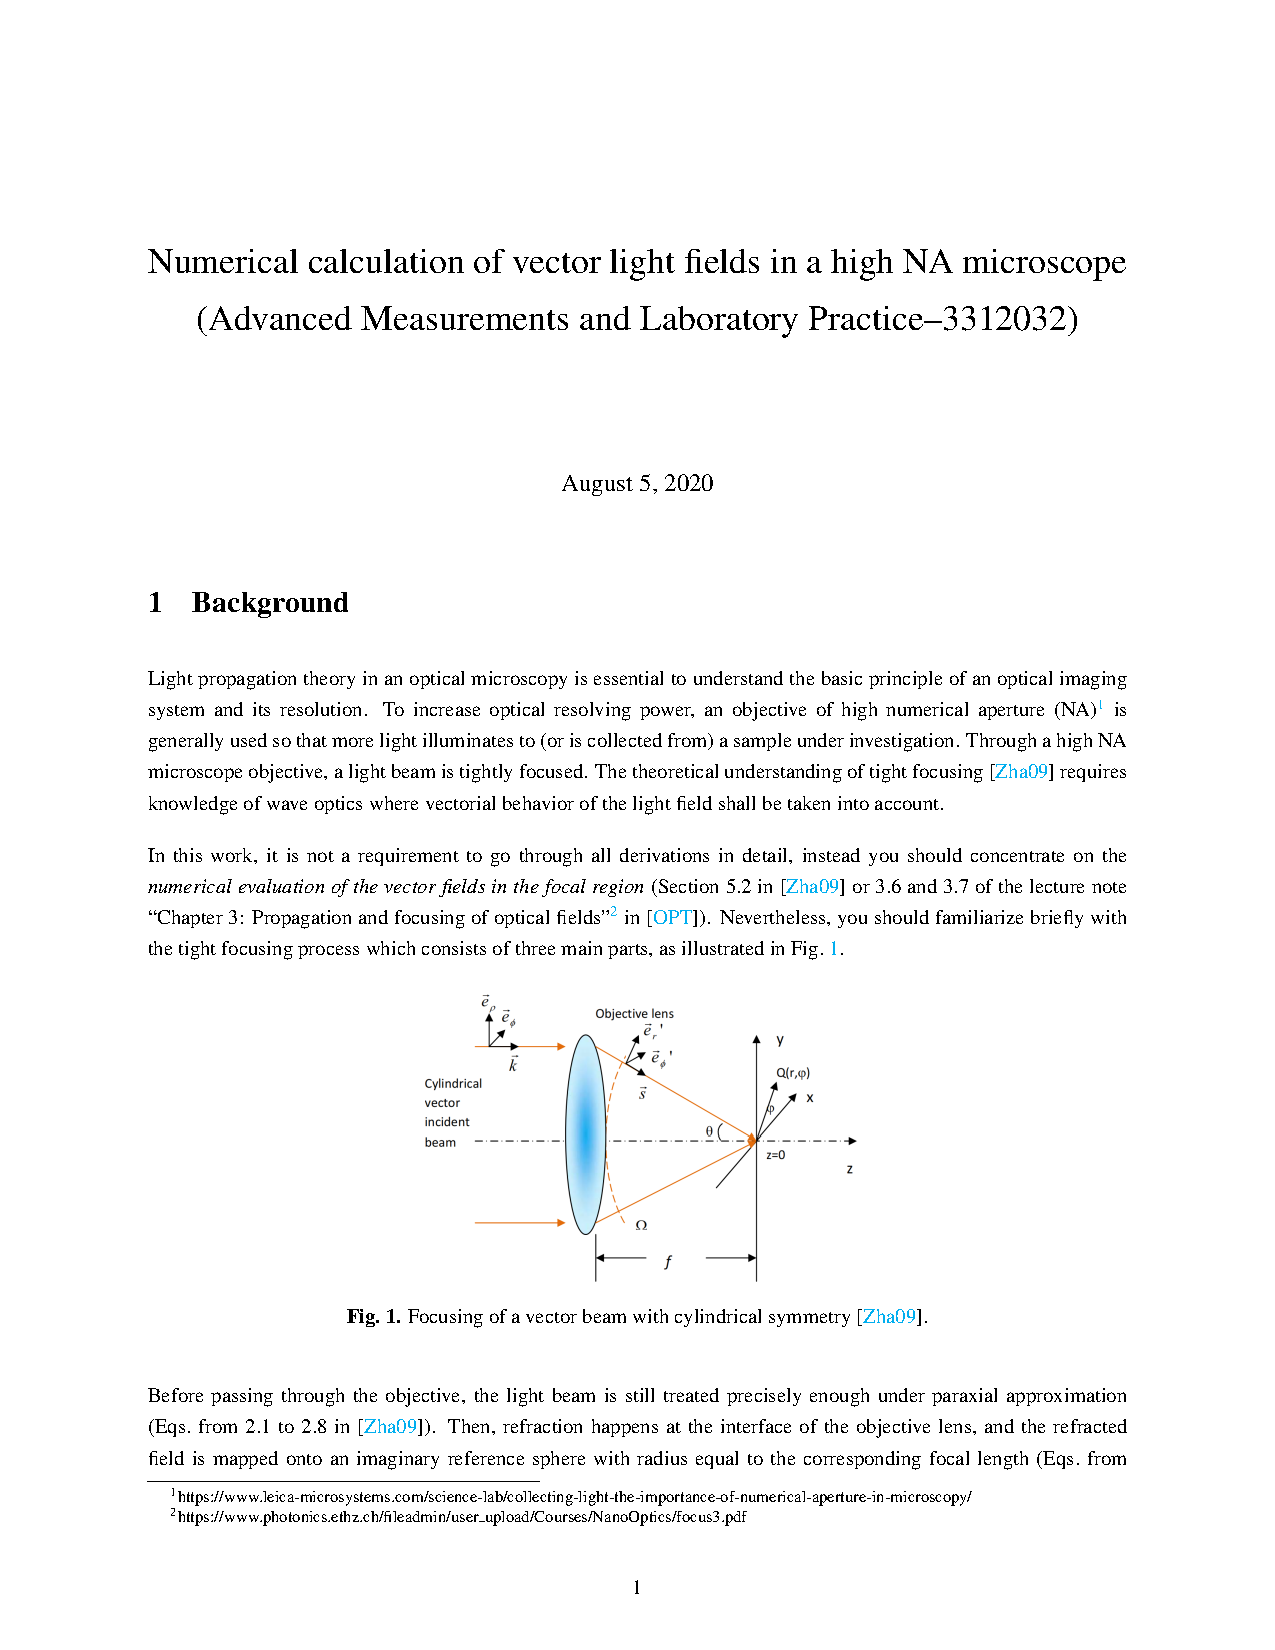
\includepdf[pages = 1-5]{NumericalVectorFieldCalculations}

\end{document}